\documentclass{article}

% Language setting
% Replace `english' with e.g. `spanish' to change the document language
\usepackage[english]{babel}

% Set page size and margins
% Replace `letterpaper' with `a4paper' for UK/EU standard size
\usepackage[letterpaper,top=2cm,bottom=2cm,left=3cm,right=3cm,marginparwidth=1.75cm]{geometry}

% Useful packages
\usepackage{amsmath}
\usepackage{graphicx}
\usepackage[colorlinks=true, allcolors=blue]{hyperref}

\title{Laboratory Work Report: Dimension Reduction with SVD}


\begin{document}
\maketitle

\section{Introduction}

This report documents the results and analysis of laboratory work 9 on linear dimension reduction using PCA and SVD.

\section{Singular Value Decomposition (SVD)}
Singular Value Decomposition (SVD) is a fundamental technique in linear algebra with various applications, including dimensionality reduction. It decomposes a real or complex matrix \( A \) into three matrices: \( U \), \( \Sigma \), and \( V^T \), as described in Equation (1).

\[ A = U \Sigma V^T \quad (1) \]

The singular values in \( \Sigma \) represent the importance of the corresponding singular vectors in \( U \) and \( V \). Dimensionality reduction with SVD involves selecting a subset of the top \( k \) singular values and truncating \( \Sigma \), \( U \), and \( V^T \), as shown in Equation (2).

\[ A_k \approx U_k \Sigma_k V_k^T \quad (2) \]

\section{Geometric Interpretation of SVD}
In geometric terms, SVD can be viewed as rotating the data represented by \( A \) such that the principal axes align with the columns of \( U \). The singular values determine the scaling along these axes. By keeping only the top \( k \) singular values, we project the data onto the subspace spanned by the corresponding principal axes, effectively reducing dimensionality.

\section{Code Implementation}
Below is the Python code used to perform dimension reduction with PCA and SVD and visualize the results:

\begin{verbatim}
import pandas as pd
import numpy as np
import matplotlib.pyplot as plt
from sklearn.decomposition import PCA
from sklearn.preprocessing import StandardScaler
from sklearn.decomposition import TruncatedSVD
from mpl_toolkits.mplot3d import Axes3D

# Load the dataset
column_names = ['Sequence Name', 'mcg', 'gvh', 'lip', 'chg', 'aac', 'alm1', 'alm2', 'class']
data = pd.read_csv('ecoli.data', sep='\s+', header=None, names=column_names)

# Prepare the data
X = data.iloc[:, 1:8].values  
y = data['class'].values 

# Standardize the data
scaler = StandardScaler()
X_scaled = scaler.fit_transform(X)

# Function to visualize results
def plot_2d(X, y, title):
    plt.figure(figsize=(10, 8))
    unique_classes = np.unique(y)
    for cls in unique_classes:
        plt.scatter(X[y == cls, 0], X[y == cls, 1], label=cls)
    plt.title(title)
    plt.legend()
    plt.show()

def plot_3d(X, y, title):
    fig = plt.figure(figsize=(10, 8))
    ax = fig.add_subplot(111, projection='3d')
    unique_classes = np.unique(y)
    for cls in unique_classes:
        ax.scatter(X[y == cls, 0], X[y == cls, 1], X[y == cls, 2], label=cls)
    ax.set_title(title)
    ax.legend()
    plt.show()

# PCA dimensionality reduction to 2D
pca_2d = PCA(n_components=2)
X_pca_2d = pca_2d.fit_transform(X_scaled)
plot_2d(X_pca_2d, y, 'PCA 2D')

# PCA dimensionality reduction to 3D
pca_3d = PCA(n_components=3)
X_pca_3d = pca_3d.fit_transform(X_scaled)
plot_3d(X_pca_3d, y, 'PCA 3D')

# SVD (TruncatedSVD) dimensionality reduction to 2D
svd_2d = TruncatedSVD(n_components=2)
X_svd_2d = svd_2d.fit_transform(X_scaled)
plot_2d(X_svd_2d, y, 'SVD 2D')

# SVD (TruncatedSVD) dimensionality reduction to 3D
svd_3d = TruncatedSVD(n_components=3)
X_svd_3d = svd_3d.fit_transform(X_scaled)
plot_3d(X_svd_3d, y, 'SVD 3D')

# Check explained variance ratio for PCA
print("PCA explained variance ratio (2D):", np.sum(pca_2d.explained_variance_ratio_))
print("PCA explained variance ratio (3D):", np.sum(pca_3d.explained_variance_ratio_))
\end{verbatim}

\section{Results}
Are shown in Figure 1 and Figure 2.
\begin{figure}[h]
    \centering
    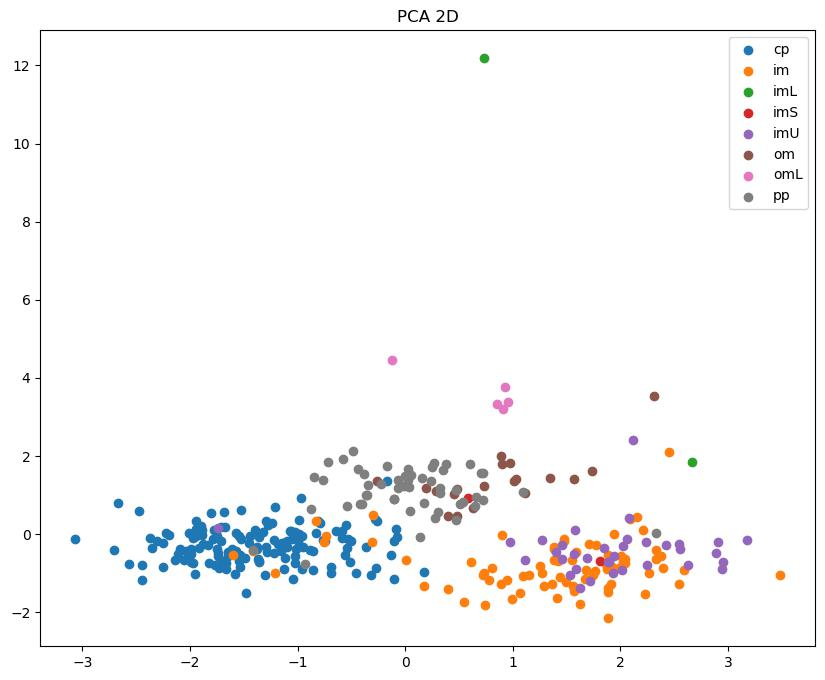
\includegraphics[width=0.8\textwidth]{pca_2d.jpg}
    \caption{PCA 2D Visualization}
\end{figure}





\section{Conclusion}
This laboratory work provided insights into the concept of Singular Value Decomposition (SVD) and its application in dimensionality reduction. Understanding SVD is essential for various data analysis tasks, including principal component analysis (PCA) and latent semantic analysis (LSA).


\end{document}
